\chapter[Particle model optimization]{Friction-limited particle with and without rate-limitation}
Investigating the friction-limited particle and the friction-limited particle with rate-limited direction control. 

The optimization problems follow the following general equation structure: 
\begin{align}
    & \underset{u}{\text{Min}}
    & & J\\
%
    & \text{subject to} 
    & & f_u(u) <= 0\\
%
    &&& f_o(x,u) <= 0 \\
%
    &&& \dot x = f(x,u),\\
%
    &&& x_0,\ x_f,
\end{align}
where $u$ is(are) the optimization variable(s), $J$ is the cost function, $f_u(u) <= 0$ and $f_o(x,u) <= 0$ denote the constraints on the controls $u$ and the states $x$, $\dot x = f(x,u)$ are the ODEs or dynamic constraints, and $x_0,\ \&\ x_f$ are the boundry conditions. 

\begin{description}
    \item[Opimization variables:] the longitudinal and lateral forces $u_x$ and $u_y$ on the vehicle. 
    \item[Cost function:] to minimize time $t$.
    \item[Constraints:] The forces on the vehicle are limited elliptically, i.e., \begin{equation*}
        u_x^2 + u_y^2 \leq (\mu m g)^2.
    \end{equation*}
    The force limit on the vehicle for the rate-limited direction control is given by \begin{align*}
        u_1^2 \leq (\mu m g)^2.
    \end{align*}\par The obstacle is given by 
    \begin{align*}
        \left(\frac{x - X_a}{R_1}\right)^n + \left(\frac{y}{R_2}\right)^n \geq 1
    \end{align*}
    \item[Vehicle model:] The friction-limited particle is given as follows: \begin{align*}
        \dot x &= v_x, \\
        \dot x &= v_x, \\
        m\,\dot v_x &= u_x,\\
        m\,\dot v_x &= u_y. \\
    \end{align*}
    The friction-limited particle with rate-limited direction control is given as follows: \begin{align*}
        \dot x &= v_x, \\
        \dot x &= v_x, \\
        m\,\dot v_x &= u_1\,\cos\left(\delta\right),\\
        m\,\dot v_y &= u_1\,\sin\left(\delta\right), \\
        \dot \delta &= u_2. \\
    \end{align*}
    \item[Miscellaneous constraints:] To ensure that the solution is within the desired operating space, certain miscellaneous constraints are included such as, \begin{align*}
        x_0 \leq x \leq x_f\\
        y_0 \leq y \leq y_f\\
        y_{min} \leq y \leq y_{max} \\
        0 \leq v_x 
    \end{align*} 
    For the rate-limited direction control model, the steering angle and steering rate is also constrained, i.e., \begin{align*}
        |\delta| \leq \delta_{max}, \\
        |\dot\delta| \leq \dot\delta_{max}, \\
    \end{align*}
\end{description}

The model, optimization, and obstacle parameters are presented in Tables~\ref{tab:flp_mdlparams},~\ref{sub@tab:flp_optparams}, and~\ref{sub@tab:flp_obsparams}, respectively. 

\begin{table}[h!]
    \begin{subtable}[h]{0.3\textwidth}
        \centering
        \begin{tabular}{c|c}
            - & value \\
            \hline
            $m$ & 500\,kg\\
            $g$ & 9.8\,m/s\textsuperscript{2}\\
            $\mu$ & 0.8\\
        \end{tabular}
        \caption{Model parameters}
        \label{tab:flp_mdlparams}
    \end{subtable}
    \hfill
    \begin{subtable}[h]{0.3\textwidth}
        \centering
        \begin{tabular}{c|c}
            - & value \\
            \hline
            $x_0$ & 0\,m\\
            $x_f$ & 100\,m\\
            $y_0$ \& $y_f$ & 1\,m\\
            $v_x$ & 40\,km/h\\
            $v_y$ & 0\,km/h
        \end{tabular}
        \caption{Optimization parameters}
        \label{tab:flp_optparams}
    \end{subtable}
    \hfill
    \begin{subtable}[h]{0.3\textwidth}
        \centering
        \begin{tabular}{c|c}
            - & value \\
            \hline
            $X_a$ & 50\,m\\
            $R_1$ & 2\,m\\
            $R_2$ & 1.5\,m\\
            $n$ & 6\\
        \end{tabular}
        \caption{Obstacle parameters}
        \label{tab:flp_obsparams}
    \end{subtable}
    \caption{Model, optimization, and obstacle parameters.}
    \label{tab:temps}
\end{table}

The optimal control problem (OCP), is solved with direct multiple-shooting with 40 control intervals for the optimization using Matlab and CasADi. The ODE was solved using the fixed-step Runge-Kutta 4 integration method. 

The results of the optimization are presented in 

\begin{figure}[h!]
    \centering
    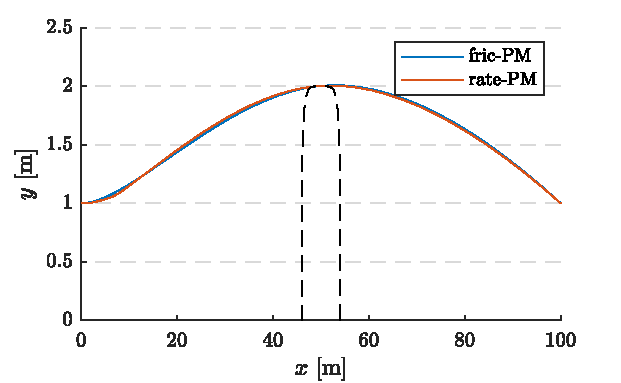
\includegraphics{figures/flp_avoid.pdf}
    \caption{Obstacle avoidance trajectory for the friction- and rate-limited particle model.}
    \label{fig:res_traj_p1}
\end{figure}

\pagebreak

\begin{table}[h]
    \centering
    \begin{tabular}{c|c|c}
        - & min $t$ & min $-v_f$ \\
        \hline
        $t$ & 3.83\,s & 3.94\,s \\
        $v_x(t_f)$ & 147.59\,km/h & 146.03\,km/h\\
    \end{tabular}
    \caption{Results for friction-limited and rate-limited particle model.}
    \label{tab:prob1_res}
\end{table}

From Table~\ref{tab:prob1_res}, it is clear that the friction-limited particle model (fric-PM) is slightly faster than the rate-limited particle model (rate-PM). 
This is because in rate-PM the rate of change of direction of the particle is limited and as a result, the ability of the vehicle to make a sharp turn is restricted and thus takes a longer time to complete the maneuver. 
This is visible in the control signals and state variables for the optimal trajectory shown in Figure~\ref{fig:prob1_res_detail}. 

Additional constraints and initial values for the firc-PM and rate-PM are presented in Table~\ref{tab:const_p1}. 

\begin{table}[h]
    \centering
    \begin{subtable}[h]{0.4\textwidth}
        \begin{tabular}{c|c||c|c}
            \multicolumn{2}{c||}{fric-PM} & \multicolumn{2}{c}{rate-PM}\\
            \hline
            $y_{max}$ & 5 & $\delta_{max}$ & $\pi/2$ \\
            - & - & $\dot\delta_{max}$ & $\pi/6$ 
        \end{tabular}
        \caption{Constraints.}
        \label{tab:const_p1a}
    \end{subtable}
    % \hfill
    \begin{subtable}[h]{0.4\textwidth}
        \begin{tabular}{c|c||c|c}
            \multicolumn{2}{c||}{fric-PM} & \multicolumn{2}{c}{rate-PM}\\
            \hline
            $v_x$ & 40\,km/h & $v_x$ & 40\,km/h
        \end{tabular}
        \caption{Initial conditions.}
        \label{tab:const_p1a}
    \end{subtable}
    \caption{Constraints for the fric-PM and rate-PM.}
    \label{tab:const_p1}
\end{table}

\begin{figure}[h!]
    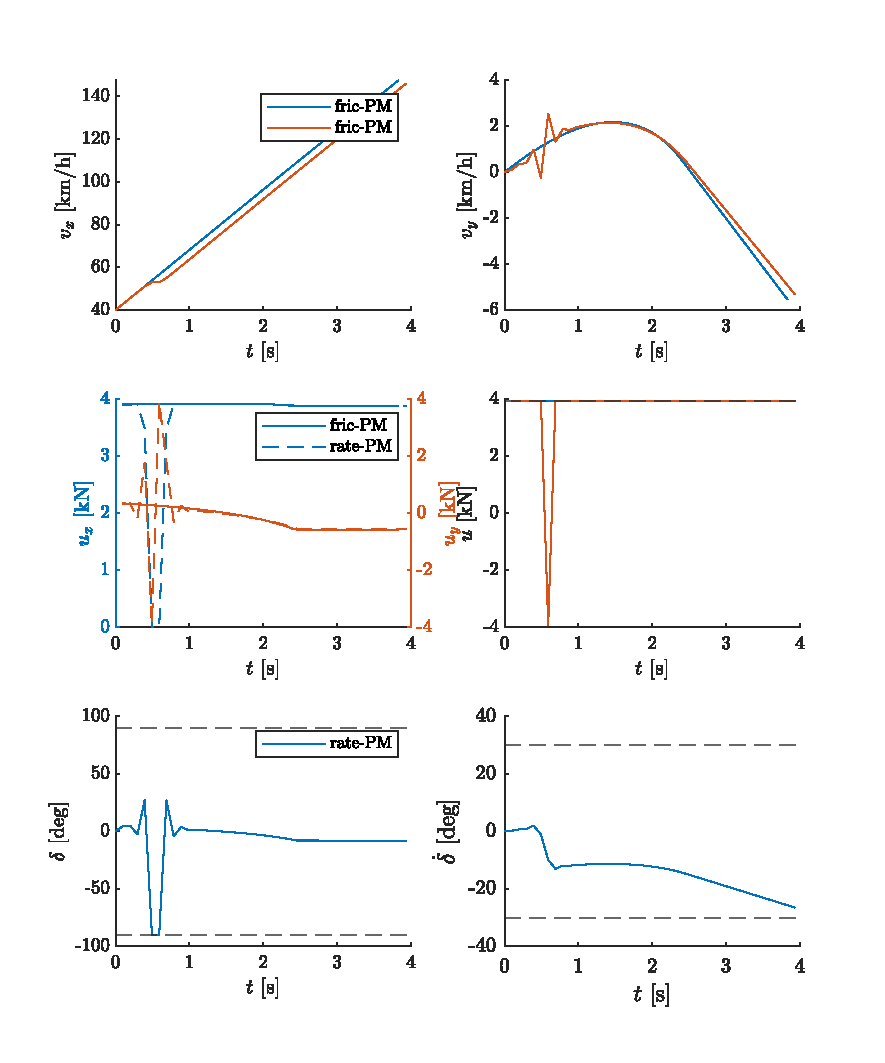
\includegraphics{figures/flp_avoid_detailed.pdf}
    \caption{Detailed optimal trajectory states and control inputs for friction- and rate-limited particle models.}
    \label{fig:prob1_res_detail}
\end{figure}

\noindent\fbox{%
    \parbox{\textwidth}{%
        \textbf{Some reflections}: \newline
        The fric-PM can converge faster than the rate-PM in some cases. 
        Since 'ipopt' is used to solve the optimization problem, fric-PM is more sensitive toward the initializations (initial guesses). 
        Therefore, additional constraints may be necessary to improve convergence.
        Furthermore, the rate-PM does not have this problem and thus can have a lower computational time.
        However, the computational time can get long with 'bad' initialization conditions. 
        The convergence of this model seems better than the fric-PM.
        
        It is worth mentioning that the terms 'improved convergence' and 'better convergence' mean the ability of the solver to produce an 'optimal solution found' even with ridiculous guesses. 
    }%
}

\section{Code}
The source codes for this problem can be found at \newline \href{https://github.com/arvba41/optimal_vehicle_maneuvers/tree/main/uppgift/ugf1}{https://github.com/arvba41/optimal\_vehicle\_maneuvers}.